\section{Evaluations}
\label{sec:eval}

We conducted three evaluations to show the effectiveness of our approach in generating regression tests that achieve a high coverage of the code under test. Our empirical results show that our approach is scalable and can automatically generate tests for large real-word applications without any manual efforts. In our evaluations,  we use two core .NET 2.0 framework libraries\footnote{\url{http://msdn.microsoft.com/en-us/library/ms229335.aspx}} as subject applications. We next describe the research questions addressed in our evaluation and present our evaluation results.

%\begin{figure*}[t]
%\centering
%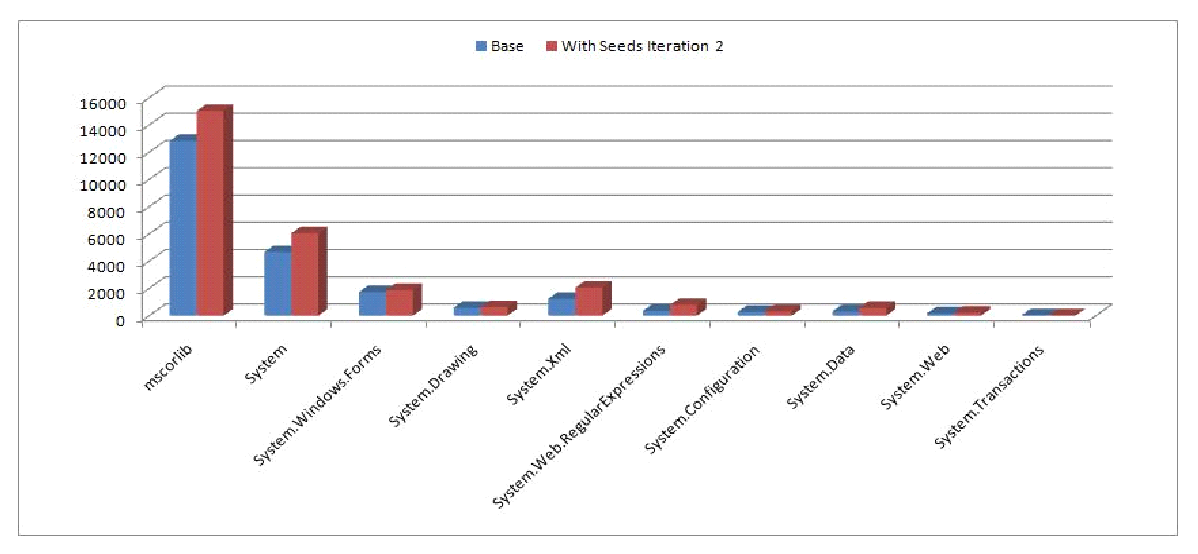
\includegraphics[scale=0.70,clip]{figs/RQ2_1.eps}\vspace*{-1ex}
%\caption{Comparison of base coverage and coverage achieved by regression tests of Mode 4 (WithSeeds Iteration 2).} \label{fig:rq2}
%\end{figure*}

%---------------------------------------------------------------------------------------
\subsection{Research Questions}
\label{sec:research}

We address the following three research questions in our evaluations.

\begin{itemize}
\item RQ1: Can our approach handle large real-world applications in automatically generating regression tests that achieve a high coverage of the code under test? 
\item RQ2: Do seed tests help achieve higher coverage of the code under test than without using seed tests?
\item RQ3: Can more machine power help generate new regression tests that can achieve more coverage of the code under test?
\end{itemize}

%---------------------------------------------------------------------------------------
\subsection{Subject Applications}

We used two core .NET 2.0 framework base class libraries as subject applications in our evaluations. We selected these libraries because these libraries are shipped and maintained in different distributions such as Version 2 and Version 4 of the ``desktop CLR'', 32-bit/64-bit Silverlight, and .NET compact framework. Therefore, it is paramount for the .NET product group to maintain identical behavior and detect any new defects between different versions of these base class libraries. Table~\ref{tab:subjects} shows the two libraries (mscorlib and System) used in our evaluations and their characteristics such as the number of classes and methods. The table also shows statistics of eight other libraries of .NET 2.0 framework. Although these other eight libraries are not our primary targets for generating regression tests, our generated regression tests include methods from these libraries since these libraries are developed based on the two core libraries: mscorlib and System. In our evaluations, we use these additional eight libraries also while presenting our coverage results. The table shows that these libraries include $0$ LOC with $0$ classes and $0$ methods.

\setlength{\tabcolsep}{1pt}
\begin{table}[t]
\begin{SmallOut}
\begin{CodeOut}
\begin{center}
\begin {tabular} {|l|c|c|c|}
\hline
\textbf{.NET libraries} & \textbf{LOC} & \textbf{\# public} & \textbf{\# public}\\ 
 & & \textbf{classes} & \textbf{methods}\\ 
\hline
\hline  mscorlib & 185K & 1440 & 17800 \\
\hline  System & & & \\
\hline  System.Windows.Forms & & & \\
\hline  System.Drawing & & & \\
\hline  System.Xml & 150K & 686 & 9920 \\
\hline  System.Web.RegularExpressions & & & \\
\hline  System.Configuration & & & \\
\hline  System.Data & 196K & 648 & 11550 \\
\hline  System.Web &  & & \\
\hline  System.Transactions & & & \\
\hline \textbf{TOTAL} &  &  &   \\
\hline
\end{tabular}
\end{center}
\end{CodeOut}
\end{SmallOut}\vspace*{-4ex}
\centering \caption {\label{tab:subjects}Ten .NET framework base class libraries used in our evaluations}
\end{table}

%---------------------------------------------------------------------------------------
\subsection{Evaluation Setup}

In our approach, we used nine machines that can be classified into three configuration categories. On each machine, we launched multiple Pex processes. The number of processes launched on a machine is based on the configuration of the machine. For example, on an eight core machine, we launched seven Pex processes. Each Pex process was exploring one class (including multiple PUTs) at a time. Table~\ref{tab:mconfig} shows all three configuration categories. The table also shows the number of machines of each configuration and the number of Pex processes launched on each machine.

\setlength{\tabcolsep}{1pt}
\begin{table}[t]
\begin{SmallOut}
\begin{CodeOut}
\begin{center}
\begin {tabular} {|l|c|c|}
\hline
\textbf{Machine Configuration} & \textbf{\# of} & \textbf{\# of} \\  
 & \textbf{machines} & \textbf{processes}\\  
\hline
\hline  Xeon 2 CPU @ 2.50 GHz, 8 cores & 1 & 7\\
				16 GB RAM & & \\
\hline  Quad core 2 CPU @ 1.90 GHz, 8 cores& 2 & 7\\
				8 GB RAM & & \\
\hline  Intel Xeon CPU @2.40 GHz, 2 cores& 6 & 1\\
				1 GB RAM & & \\
\hline
\end{tabular}
\end{center}
\end{CodeOut}
\end{SmallOut}\vspace*{-4ex}
\centering \caption {\label{tab:mconfig}Three categories of machine configurations used in our evaluations.}
\end{table}

As we used .NET framework base class libraries in our evaluations, the generated tests may invoke method calls that can can cause external side effects, and change the machine configuration. Therefore, while executing the code during exploration of PUTs or while running generated tests, we created a sand-box with the ``Internet'' security permission. This permission represents the default policy permission set for the content from an unknown origin. This permission blocks all operations that involve environment interactions such as file creations or registry accesses by throwing \CodeIn{SecurityException}. Since we use sand-box in our evaluations, the reported coverage is lower than the actual coverage that can be achieved by our generated regression tests.

To address our research questions, we first created a base line in terms of the code coverage achieved by the seed tests, referred to as \emph{base coverage}. In our evaluations, we use block coverage (Section~\ref{sec:blockcov}) as a coverage criteria. We report our coverage in terms of the number of blocks covered in the code under test. We don't give an upper bound on the number of reachable basic blocks, as we don't know which blocks are actually reachable from the given scenarios.

We next generated regression tests in four different modes. In Mode 1 (referred to as \emph{WithoutSeeds Iteration 1}), we generated regression tests without using seed tests for one iteration. In Mode 2 (referred to as \emph{WithoutSeeds Iteration 2}), we generated regression tests without using seed tests for two iterations. The regression tests generated in Mode 2 are a super set of the regression tests generated in Mode 1. In Mode 3 (referred to as \emph{WithSeeds Iteration 1}), we generated regression tests with using seed tests for one iteration. Finally, in Mode 4 (referred to as \emph{WithSeeds Iteration 2}), we generated regression tests with using seed tests for two iterations. Modes 1 and 3 took one and half day for generating tests, whereas Modes 2 and 4 took three days since these modes correspond to Iteration 2.

\setlength{\tabcolsep}{1pt}
\begin{table}[t]
\begin{SmallOut}
\begin{CodeOut}
\begin{center}
\begin {tabular} {|l|c|c|c|}
\hline
\textbf{Mode} & \textbf{\# of} & \textbf{\# of covered} & \textbf{\% of increase}\\  
 & \textbf{Tests} & \textbf{blocks} & \textbf{from base}\\  
\hline
\hline  WithoutSeeds Iteration 1 & 248,306 & 21,920 & 0\%\\
\hline  WithoutSeeds Iteration 2 & 412,928 & 23,176 & 4.8\%\\
\hline  WithSeeds Iteration 1 & 376,367 & 26,939 & 21.8\%\\
\hline  WithSeeds Iteration 2 & 501,799 & 27,485 & 24.3\%\\
\hline
\end{tabular}
\end{center}
\end{CodeOut}
\end{SmallOut}\vspace*{-4ex}
\centering \caption {\label{tab:gentests}Generated regression tests.}
\end{table}

%---------------------------------------------------------------------------------------
\subsection{RQ1: Generated Regression Tests}

We next address the first research question of whether our approach can handle large real-world applications in automatically generating regression tests. This research question helps to show that our approach can be used in practice and can address scalability issues in generating regression tests for large applications. We first present the statistics after each phase in our approach and next present the number of regression tests generated in each mode.

In the capture phase, our approach recorded $\approx$1.50 GB C\# source code (including 433,809 traces) of dynamic traces for the two libraries. The average trace length includes $21$ method calls and the maximum trace length includes $52$ method calls. As our capture phase transforms each dynamic trace into a PUT and a seed test, the capture phase resulted in 433,809 PUTs and 433,809 seed tests. 

In the minimize phase, our approach uses static analysis to filter out duplicate PUTs. Our static analysis took 45 minutes and resulted in 68,575 unique PUTs. Our approach uses dynamic analysis to filter our duplicate seed tests. Our dynamic analysis took 5 hours and resulted in 128,185 unique seed tests. These results show that there are a large number of duplicate PUTs and seed tests, and show the significance of our minimize phase. We next measured the block coverage achieved by these 128,185 unique seed tests in the code under test and used this coverage as \emph{base coverage}. These tests covered 22,111 blocks in the code under test. 

Table~\ref{tab:gentests} shows the number of regression tests generated in each mode along with the number of covered blocks. The table also shows the percentage of increase
in the number of blocks compared to the base coverage. As shown in results, in Mode 4 (WithSeeds Iteration 2), our approach achieved 24.3\% higher coverage than the base coverage. Table~\ref{tab:detailedres} shows more detailed results of coverages achieved for all ten .NET libraries. Column ``.NET libraries'' shows the library under test. Column ``Base Coverage'' shows the number of blocks covered by seed tests for each library. Column ``WithOutSeeds Iteration 1'' shows the number of blocks covered (``\# blocks'') and the percentage of increase in the coverage (``\% increase'') with respect to the base coverage in this mode. Similarly, Columns ``WithOutSeeds Iteration 2'', ``WithSeeds Iteration 1'', and ``WithSeeds Iteration 2'' show the results of the other three modes. 

As we use seed tests during our exploration in Mode ``WithSeeds Iteration 2'', the coverage achieved is either the same or higher than the base coverage. However, our approach has achieved significant higher coverages than base coverage for libraries mscorlib and System (in terms of the number of additional blocks covered). The primary reason is that most of the classes in these libraries are stateless and do not require environment interactions. The results show that our approach can handle large real-world applications and can generate large number of regression tests that achieve a high coverage of the code under test.

\setlength{\tabcolsep}{1pt}
\begin{table*}[t]
\begin{SmallOut}
\begin{CodeOut}
\begin{center}
\begin {tabular} {|l|c|c|c|c|c|c|c|c|c|}
\hline
\textbf{.NET libraries} & \textbf{Base} & \multicolumn{2}{|c|}{\textbf{WithOutSeeds}} & \multicolumn{2}{|c|}{\textbf{WithOutSeeds}} & \multicolumn{2}{|c|}{\textbf{WithSeeds}} & \multicolumn{2}{|c|}{\textbf{WithSeeds}}\\ 
 & \textbf{Coverage} & \multicolumn{2}{|c|}{\textbf{Iteration 1}} & \multicolumn{2}{|c|}{\textbf{Iteration 2}} & \multicolumn{2}{|c|}{\textbf{Iteration 1}} & \multicolumn{2}{|c|}{\textbf{Iteration 2}}\\ 
\cline{3-10}
 & \# blocks & \# blocks & \% increase & \# blocks & \% increase & \# blocks & \% increase & \# blocks & \% increase\\ 
\hline  mscorlib   						& 12827 	& 13063 & 1.84		& 13620 & 6.18	& 14808	& 15.44		& 15018	& 17.08					\\
\hline  System    						& 4651  	& 4062  & -12.67	& 4243	& -8.77	& 5907	& 27.00		& 6039	& 29.84 				\\
\hline  System.Windows.Forms  & 1730 		& 1572  & -9.13		& 1774	& 2.54	& 1782	& 3.01		& 1865	& 7.80 					\\
\hline  System.Drawing 				& 570			& 580		& 1.75		& 591		& 3.68	& 618		& 8.42		& 625		& 9.65 					\\
\hline  System.Xml 						& 1229    & 1390	& 13.10		& 1462	& 18.96	& 1959	& 59.40		& 2045	& 66.40 				\\
\hline  System.Web.Regular 		& 351     & 330		& -5.98		& 520		& 48.15	& 754		& 114.81 	& 771		& 119.66 				\\
			  Expressions 					& 				& 			& 				& 			& 			& 			& 				& 			&  							\\
\hline  System.Configuration 	& 263 		& 297 	& 12.93		& 297		& 12.93	& 302		& 14.83		& 306		& 16.35 				\\
\hline  System.Data 					& 301 		& 380		& 26.25		& 422		& 40.20	& 562		& 86.71		& 569		& 89.04 				\\
\hline  System.Web 						& 154			& 211		& 37.01		& 212		& 37.66	& 212		& 37.66		& 212		& 37.66 				\\
\hline  System.Transactions 	& 35			& 35		& 0.00		& 35		& 0.00	& 35		& 0.00		& 35		& 0.00 					\\
\hline \textbf{TOTAL/AVERAGE} & \textbf{22111} & \textbf{21920} & \textbf{<0} & \textbf{23176} & \textbf{4.80} & \textbf{26939}	& \textbf{21.80} & \textbf{27485} & \textbf{24.30} \\
\hline
\end{tabular}
\end{center}
\end{CodeOut}
\end{SmallOut}
\centering \caption {\label{tab:detailedres}Comparison of coverages achieved for ten .NET libraries used in our evaluation.}
\end{table*}

%---------------------------------------------------------------------------------------
\subsection{RQ2: Using Seed Tests}

We next address the second research question of whether seed tests help achieve higher code coverage compared to without using seed tests. To address this question, we compare the coverages achieved by generated tests in Modes ``WithoutSeeds Iteration 2'' and ``WithSeeds Iteration 2''. As shown in Table~\ref{tab:detailedres}, Mode ``WithSeeds Iteration 2'' always achieved higher coverage than Mode ``WithoutSeeds Iteration 2''. On average ``WithSeeds Iteration 2'' achieved 18.6\% higher coverage than Mode ``WithoutSeeds Iteration 2''. The table also shows that there is a significant increase in the coverage achieved for the \CodeIn{System.Web.RegularExpressions} library. 
In Section~\ref{sec:explore}, we described one of the advantages of seed tests is that seed tests can help cover certain paths that are hard to be covered without using those tests. The \CodeIn{System.Web.RegularExpressions} library is an example for such paths since this library requires complex regular expressions to cover certain paths in the library. It is quite challenging for Pex or any other dynamic-symbolic-execution-based approach to generate concrete values that represent regular expressions. Therefore, concrete values in the seed tests helped achieve higher coverage for this library. In summary, the results show that seed tests help achieve higher coverages compared to without using seed tests.

%\begin{figure*}[t]
%\centering
%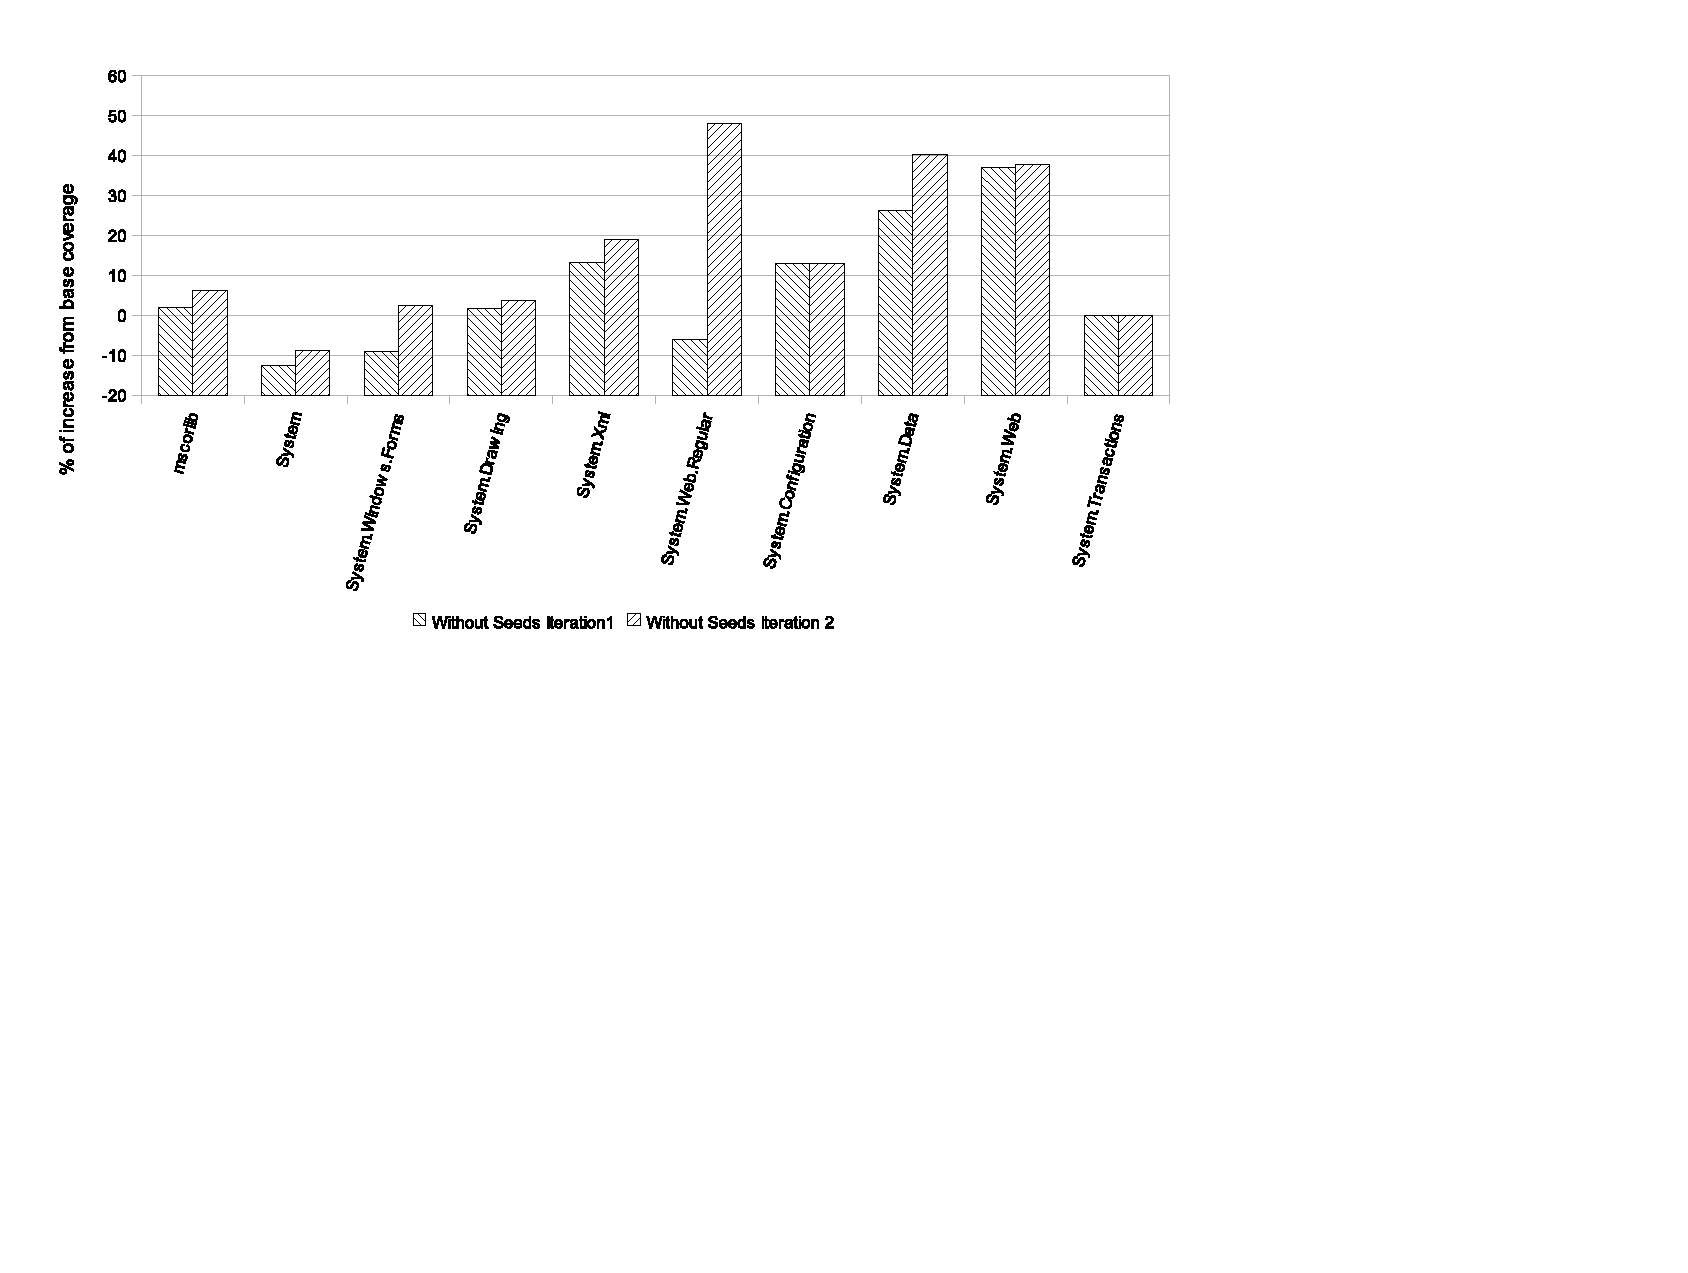
\includegraphics[scale=0.70,clip]{figs/RQ3_1.eps}\vspace*{-1ex}
%\caption{Comparison of code coverages achieved by base, Modes 2 (WithoutSeeds Iteration 2) and 4 (Withseeds Iteration 2).} \label{fig:rq3}
%\end{figure*}

%---------------------------------------------------------------------------------------
\subsection{RQ3: Using More Machine Power}

We next address the third research question of whether more machine power helps to achieve more coverage. This research question helps to show that additional coverage can be achieved in further iterations of our approach. To address this question, we compare coverages achieved in Mode ``WithoutSeeds Iteration 1'' with Mode ``WithoutSeeds Iteration 2'', and Mode ``WithSeeds Iteration 2'' with Mode ``WithSeeds Iteration 2'' (shown in Table~\ref{tab:detailedres}). 

On average, Mode ``WithoutSeeds Iteration 2'' achieved 5.73\% higher coverage than Mode 1. This result show that our approach can achieve additional coverage in further iterations. However, the coverage from Mode 1 to Mode 2 is not doubled. The primary reason is that it gets harder to cover new blocks in further iterations.

Figure~\ref{fig:rq42} shows the comparison results of Mode 3 with Mode 4. On average, Mode 4 achieved 2.0\% higher coverage than Mode 3. As shown, the increase in coverage from Mode 3 to Mode 4 is less than the increase in the coverage from Mode 1 to Mode 2. This difference is due to seed tests that help achieve higher coverage during Mode 3, leaving more harder blocks to be covered in Mode 4. In summary, the results show that further iterations can help generate new regression tests that can achieve more coverage.

\begin{figure*}[t]
\centering
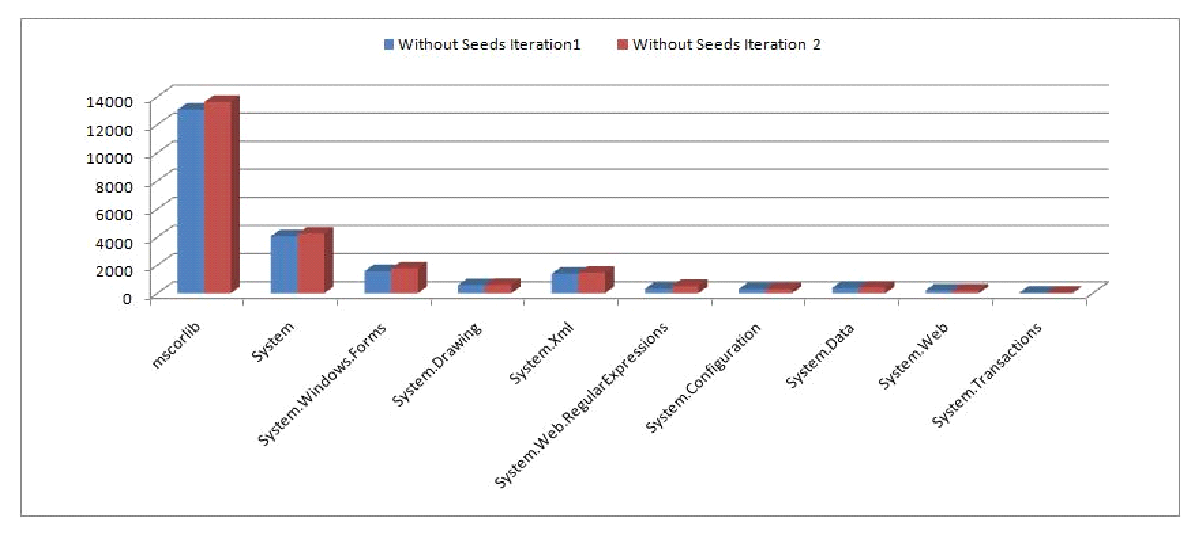
\includegraphics[scale=0.70,clip]{figs/RQ4_1_1.eps}\vspace*{-1ex}
\caption{\label{fig:rq41}Comparison of code coverages achieved by Modes 1 (WithoutSeeds Iteration 1) and 2 (WithoutSeeds Iteration 2).} 
\end{figure*}


\begin{figure*}[t]
\centering
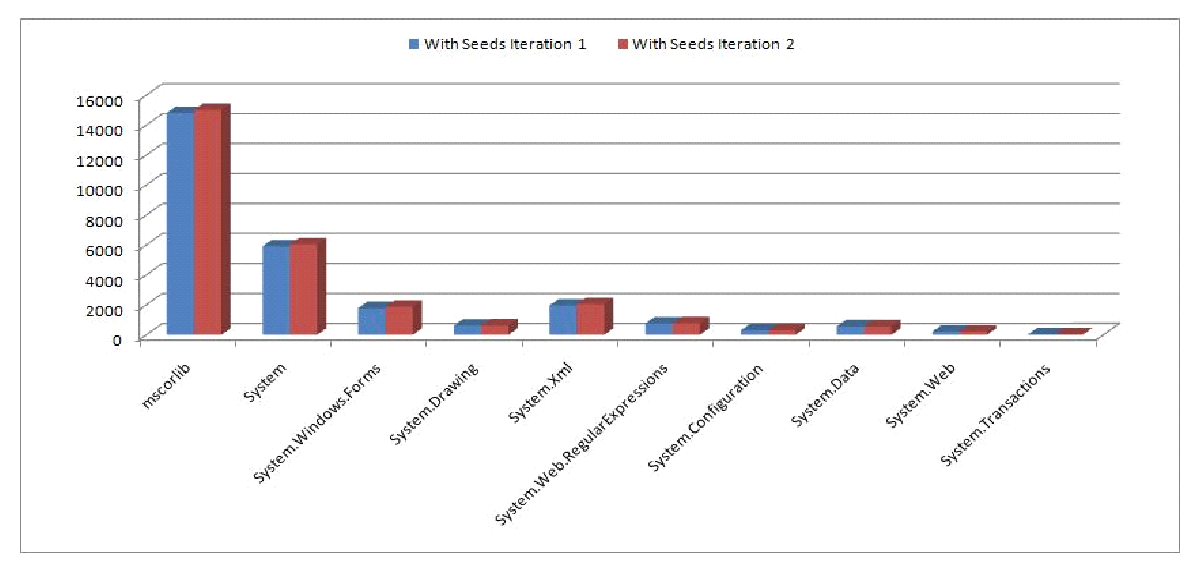
\includegraphics[scale=0.70,clip]{figs/RQ4_2_1.eps}\vspace*{-1ex}
\caption{\label{fig:rq42}Comparison of code coverages achieved by Modes 3 (WithSeeds Iteration 1) and 4 (Withseeds Iteration 2).}
\end{figure*}


%---------------------------------------------------------------------------------------
%\subsection{Real Defects}

%Our approach automatically generates test scenarios from dynamic traces. We use these test scenarios
%in generating PUTs and then generating regression tests on a stable versions. These regression tests
%can be used on future versions to detect regression faults. In our approach, we cannot detect
%defects in the version on which regression tests generated because of lack of test oracles. However,
%we identify that many exceptions are observed while generating regression tests on the version.
%We next describe the raised exceptions and describe more about the defects detected.